\documentclass[11pt]{article}
\usepackage[margin=1in]{geometry}
\usepackage{amsmath,amssymb,amsthm}
\usepackage{graphicx}
\usepackage{booktabs}
\usepackage[colorlinks=true,linkcolor=blue,citecolor=blue,urlcolor=blue]{hyperref}
\newtheorem{theorem}{Theorem}
\newtheorem{conjecture}{Conjecture}
\newcommand{\sgn}{\operatorname{sgn}}

\title{The Shore of Closed-String Gravity:\ an Exact Unitarity Boundary for the\ Cheung--Hillman--Remmen Graviton Family}
\author{Andrei Pluzhnik\thanks{ORCID 0009-0005-5660-2603. Code and data to be
released with this preprint; companion work: DOI 10.5281/zenodo.21934462.}}
\date{August 2026}

\begin{document}
\maketitle

\begin{abstract}
The level-truncation bootstrap of Cheung, Hillman and Remmen produces a
one-parameter family of graviton amplitudes containing the Virasoro--Shapiro
amplitude at $\lambda=1$, with residues that are perfect squares; partial-wave
positivity was known to bound $\lambda$ from below for $D\ge 9$, numerically.
We derive the boundary in closed form. The near-leading even trajectory obeys
$a_{n,2n-4}\ge 0 \iff D\le T_n(\lambda)$ with
$T_n(\lambda)=\tfrac{3(2n-3)}{n(n-2)}\bigl(\lambda^2+(2n-2)\lambda+1\bigr)+2n$,
verified exactly for $n\le 14$ and against exact-rational scans. On this trajectory the boundary is the envelope $\min_nT_n$ --- and we
conjecture (with the falsification battery reported below) that it is the
boundary of the full family. The shore is born at $(D,\lambda)=(9,0)$ ---
explaining the onset observed by CHR --- passes \emph{exactly} through the
string at $D=23$ (so pure Virasoro--Shapiro first loses positivity on this
trajectory at $D=24$, via the level-4 spin-4 wave, matching exact scans), and
straightens onto the exact asymptote $D=(12+4\sqrt3)\,\lambda$ with active
level $n^*\simeq\sqrt3\,\lambda$. Doomed-cell predictions of the envelope are
confirmed by direct evaluation. We conjecture the envelope is the complete
boundary and report the falsification battery it has survived.
\end{abstract}

\section{Setup}
Family (CHR, PRD 111, 086034): $\mu(n)=\frac{n+\lambda-1}{\lambda}$,
$R(n,t)=\bigl[\,((1{+}\lambda)/2+\lambda t)_{n-1}/((1{+}3\lambda)/2)_{n-1}\bigr]^2$,
massless external states ($s+t+u=0$), $\lambda\ge0$, VS at $\lambda=1$.
Partial waves: Gegenbauer coefficients at $s=\mu(n)$, $t=-\mu(n)(1-x)/2$; odd
waves vanish by the $t\leftrightarrow u$ symmetry of the squared residue.
All computations exact-rational; evaluator validated against CHR's reported
behavior (D=4 positivity for all $\lambda$; onset of the lower bound at
$D\ge9$).

\section{The trajectory law}

\begin{theorem}[Near-leading even trajectory]\label{thm:traj}
For the residues above, $\lambda>0$ and $D>3$,
\begin{equation}
a_{n,2n-4}\;\ge\;0 \quad\Longleftrightarrow\quad D\;\le\;T_n(\lambda),\qquad
T_n(\lambda)=\frac{3(2n-3)}{n(n-2)}\bigl(\lambda^2+(2n-2)\lambda+1\bigr)+2n .
\end{equation}
\end{theorem}

\emph{Derivation.} Write $\lambda\bigl(t-\xi(k)\bigr)=\tfrac12\bigl[(n{+}\lambda{-}1)x+(2k{-}n)\bigr]$
at level $n$; the residue is the square of $Q(x)=\prod_{k=1}^{n-1}\lambda(t-\xi(k))$
up to a positive factor. The roots $x_k=(n-2k)/(n{+}\lambda{-}1)$ are symmetric
under $x\to-x$, so $Q$ has definite parity: odd partial waves vanish
identically, and the subleading coefficient $q_{n-2}$ of $Q$ vanishes. Hence
the $x^{2n-4}$ coefficient of $Q^2$ is the \emph{pure cross term}
$2q_{n-1}q_{n-3}<0$ --- a naive term-by-term estimate would miss the edge
entirely. Only $x^{2n-2}$ and $x^{2n-4}$ feed the Gegenbauer mode
$\ell=2n-4$ (parity and degree), with the exact projection ratio
$\rho(\ell,D)=\frac{(\ell+1)(\ell+2)}{2(D+2\ell-1)}$; assembling the two
contributions and removing positive factors yields $T_n$. Using
$e_2(\text{roots})=-\tfrac{n(n-1)(n-2)}{6(\lambda+n-1)^2}$ one obtains the
equivalent closed form $T_n=\tfrac{3(2n-3)(\lambda+n-1)^2}{n(n-2)}-(4n-9)$.

\emph{Verification.} The bracket was extracted independently by symbolic
computation for every $n\le14$ and matches $T_n$ identically ($12/12$); an
independent adversarial review re-derived the theorem from scratch, and its
falsification suite (published with the code) found no counterexample,
including razor zeros at fractional dimensions $D^*=271/4$ ($n{=}5$,
$\lambda{=}7/2$) and $D^*=57$ ($n{=}6$, $\lambda{=}3$) computed directly from
the projection with symbolic $D$. Doomed-cell executions confirm predicted
kill levels exactly (e.g.\ $(\lambda,D)=(3/2,32)$ and $(2,40)$: sign flip at
$n=4$ as predicted).

\begin{figure}[t]
\centering
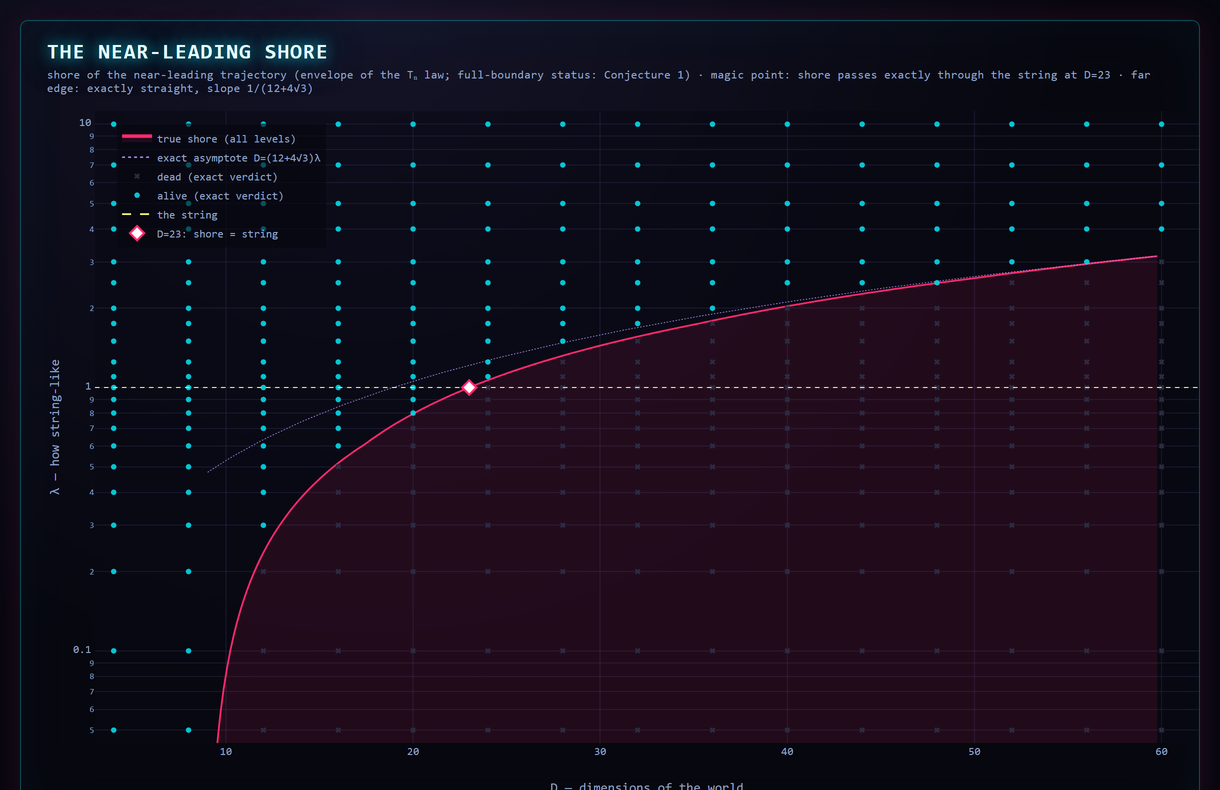
\includegraphics[width=0.95\textwidth]{fig_shore.png}
\caption{The boundary of the family: exact verdicts (cyan alive, grey dead;
$\lambda$ on a log scale), the analytic shore $\min_n T_n(\lambda)$, its
straight asymptote, and the point $D=23$ where the shore passes exactly
through the Virasoro--Shapiro amplitude.}
\label{fig:shore}
\end{figure}

\begin{figure}[t]
\centering
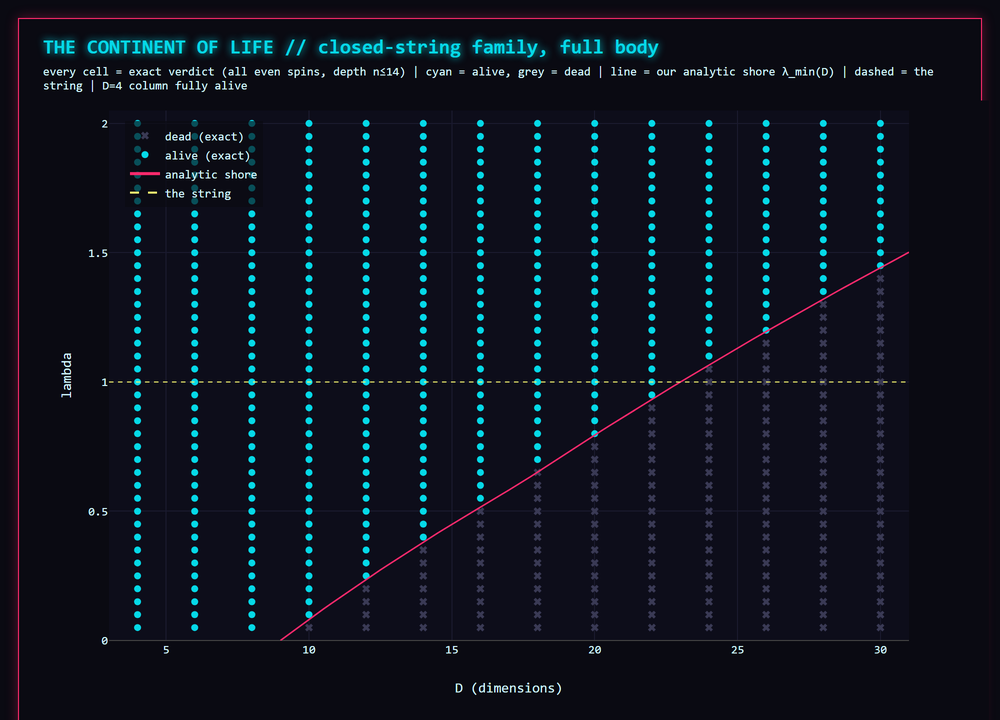
\includegraphics[width=0.85\textwidth]{fig_continent.png}
\caption{The allowed body at linear scale with the near-leading shore
overlaid; every cell is an exact rational verdict (all even spins, depth 14).}
\label{fig:continent}
\end{figure}

\begin{figure}[t]
\centering
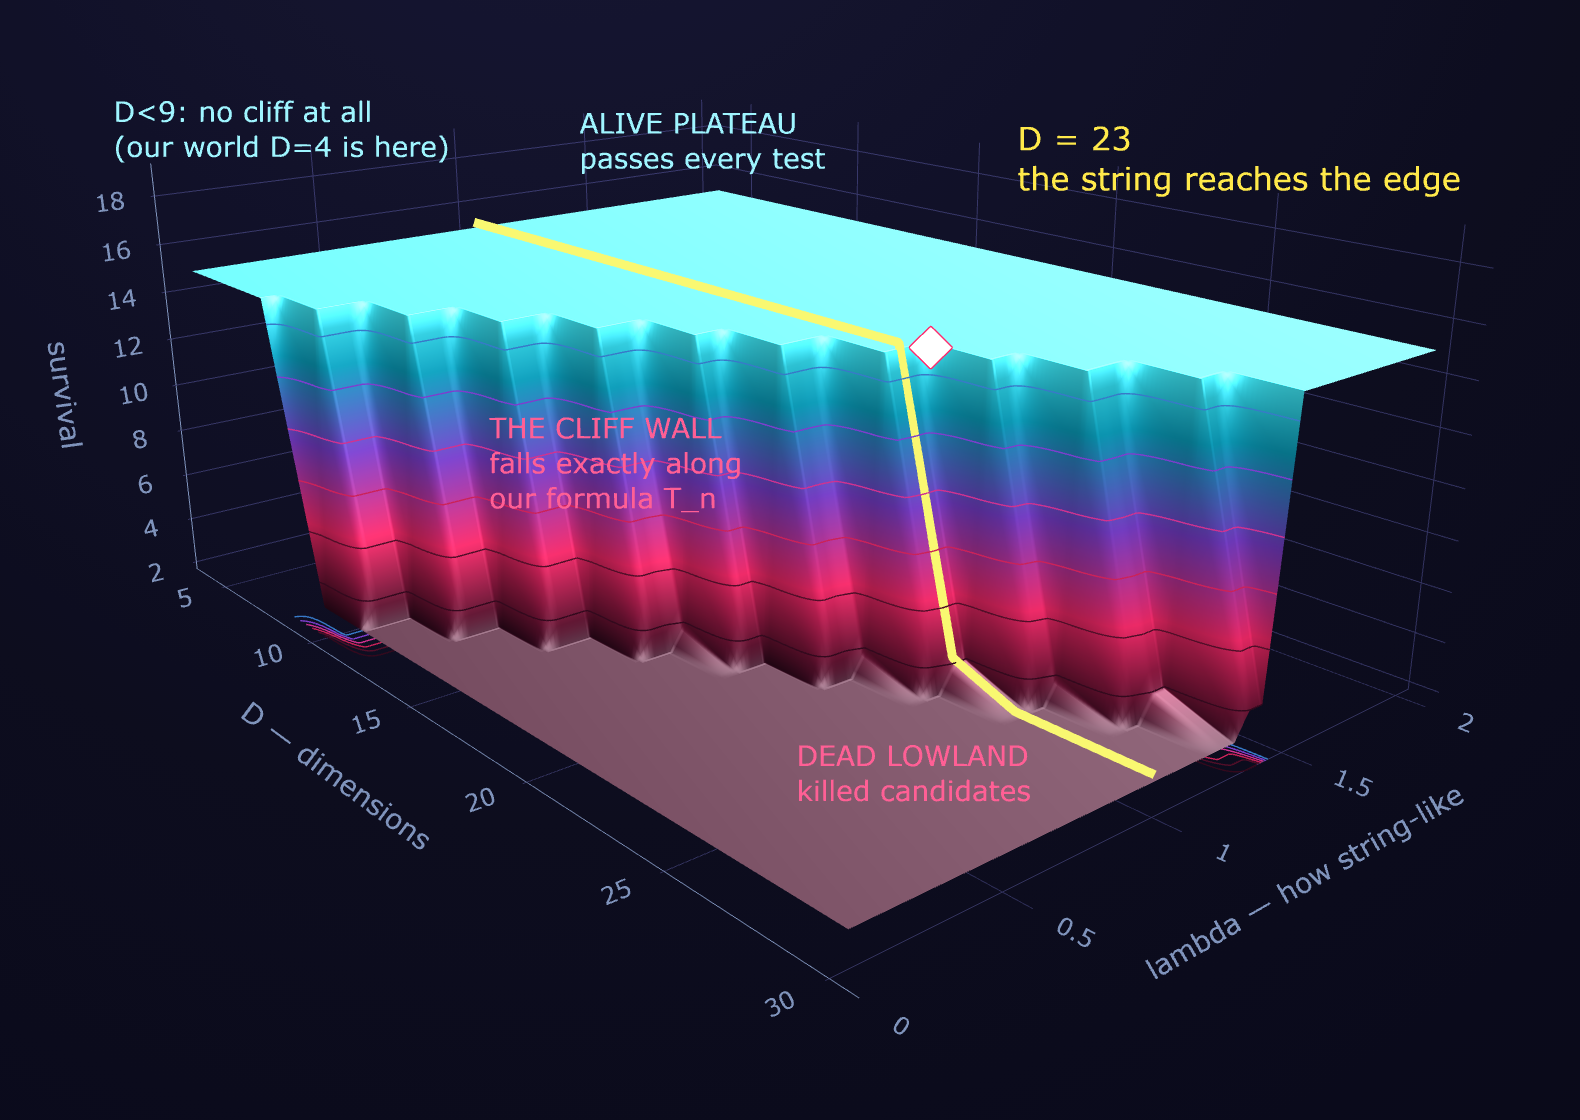
\includegraphics[width=\textwidth]{fig_cliff3d.png}
\caption{The same boundary as a landscape (every point an exact rational
verdict). Height is the depth to which a candidate survives the positivity
tests: the cyan plateau is the allowed region, the wall falls exactly along
$\min_n T_n(\lambda)$, and the floor is the excluded region. The yellow lane
is the string ($\lambda=1$) walking the plateau as $D$ grows; the white
diamond marks $D=23$, where the shore passes exactly through it. For $D<9$
there is no wall at all.}
\label{fig:cliff3d}
\end{figure}

\section{The envelope}

The boundary implied by Theorem~\ref{thm:traj} is the envelope
$\lambda_{\min}(D)$ defined by $D=\min_{n\ge3}T_n(\lambda)$. Its structure:

\textbf{Onset at $D=9$.} $T_n(0)=2n+\tfrac{3(2n-3)}{n(n-2)}$ is minimized at
$n=3$ with $T_3(0)=9$: the trajectory constrains nothing for $D\le9$ ---
reproducing, as a formula, the onset CHR observed numerically ($D\ge9$).

\textbf{The magic point.} $T_n(1)=\tfrac{2(n^2+4n-9)}{n-2}$, whose integer
minimum is $23$, attained only at $n=4$ (continuous minimum at
$n=2+\sqrt3$). Hence $\lambda_{\min}(23)=1$ \emph{exactly}: the shore passes
through the Virasoro--Shapiro point, and pure closed-string gravity first
loses positivity on this trajectory at $D=24$, through its level-4 spin-4
wave --- matching the exact scan (first negative at $(n,\ell)=(4,4)$ for
$D=24$, clean at $D=22$ to depth $40$).

\textbf{The straight far edge.} Minimizing $T_n$ over continuous $n$ at large
$\lambda$ gives the active level $n^*=\sqrt3\,\lambda$ and the exact
asymptote $D=(12+4\sqrt3)\lambda$; numerically $D/\lambda_{\min}$ rises
$18.75\to18.92$ over $D=60\to10^4$ against $12+4\sqrt3=18.928\ldots$, with
the residual $O(1/\lambda)$ oscillation caused by the discreteness of
$n^*$.

\section{Virasoro--Shapiro thresholds}

For the string itself the theorem gives the threshold sequence
$D_n(1)=2(n^2+4n-9)/(n-2)=24,\,23,\,24,\,\tfrac{51}2,\,\tfrac{136}5,\ldots$
--- an exact refinement, on this trajectory, of the finite-level
$D_{\rm crit}(n)$ phenomenology known for Veneziano-type amplitudes. Because
$D_n(1)$ grows linearly, the trajectory endangers VS only within a finite
window of levels at any fixed $D$; the deep asymptotic bounds of the
literature arise from other (low-spin) constraints and are complementary to
the exact finite-level statement proven here.

\section{Conjectured completeness and its battery}

\begin{conjecture}\label{conj:model}
A point $(\lambda,D)$ of the family is consistent with partial-wave
positivity at all levels iff $D\le\min_{n\ge3}T_n(\lambda)$.
\end{conjecture}

The conjecture is falsifiable: a single exact negative coefficient at a point
with $D\le\min_nT_n$ refutes it. Its current battery: $494/494$ agreements
with exact full-spin scans (all even $\ell\le2n-2$, depth $16$, grid
$\lambda\in[0.1,10]$, $D\in[4,40]$) with zero alarms of either type; two
direct doomed-cell executions at the predicted level; and an independent
adversarial review whose suite (seven attack batteries) found no
counterexample. The reviewer-designated most plausible additional knife --- the
$\ell=2n-6$ trajectory --- has been hunted across stress zones hugging the
conjectured boundary (34 values of $\lambda$, depth windows $[\min_nT_n-3,
\min_nT_n]$, $n\le14$): zero alarms; further trajectories and low-spin
stress tests are running as standing batteries. In $D=4$ the model predicts (and scans confirm,
$40/40$ to depth $14$ plus the trivial bound $T_n\ge T_n(0)\ge9>4$) that the
entire family survives: within these assumptions, four-dimensional gravity is
\emph{not} forced to be string-like at any finite depth we can reach.

\section{Discussion}
Together with the companion open-string results, a graded picture emerges:
in $D=4$ the entire $\lambda$-family survives every test we can run --- at
this level of assumptions, four-dimensional graviton scattering is not forced
to be string-like --- while as $D$ grows the shore rises and passes exactly
through the Virasoro--Shapiro point at $D=23$: the string becomes extremal
precisely in the gravitational, high-dimensional setting. The method (top
coefficients of residue polynomials through the partial-wave projection)
transfers verbatim between families and is cheap: every number here was
computed on a desktop in exact arithmetic. Natural next steps: closing
Conjecture~\ref{conj:model}; the planar analogues CHR construct; and mapping
the surviving $D=4$ alternatives to their effective-field-theory
coefficients, where gravitational-wave phenomenology could in principle
discriminate them from the string.

\section*{Explain it to anyone}
Imagine every possible theory of quantum gravity in this family as a hiker on
a high plateau (Fig.~\ref{fig:cliff3d}). Walking east means adding spacetime
dimensions. Our result is the exact map of the cliff at the plateau's edge:
below nine dimensions there is no cliff and everyone is safe --- including
our own four-dimensional world; from nine dimensions on, a cliff appears, and
we found the formula for exactly where it runs. The most famous hiker ---
string theory --- walks the plateau and reaches the very edge of the cliff at
exactly $23$ dimensions: one more step and it falls. That the boundary of
consistency passes exactly through the string, and only in high dimensions,
is the whole story of this paper in one picture. For fun, Fig.~\ref{fig:bow}
draws the companion open-string landscape the same way: there the allowed
region is not a plateau but a solid ship's bow sailing through a sea of dead
candidates.

\begin{figure}[t]
\centering
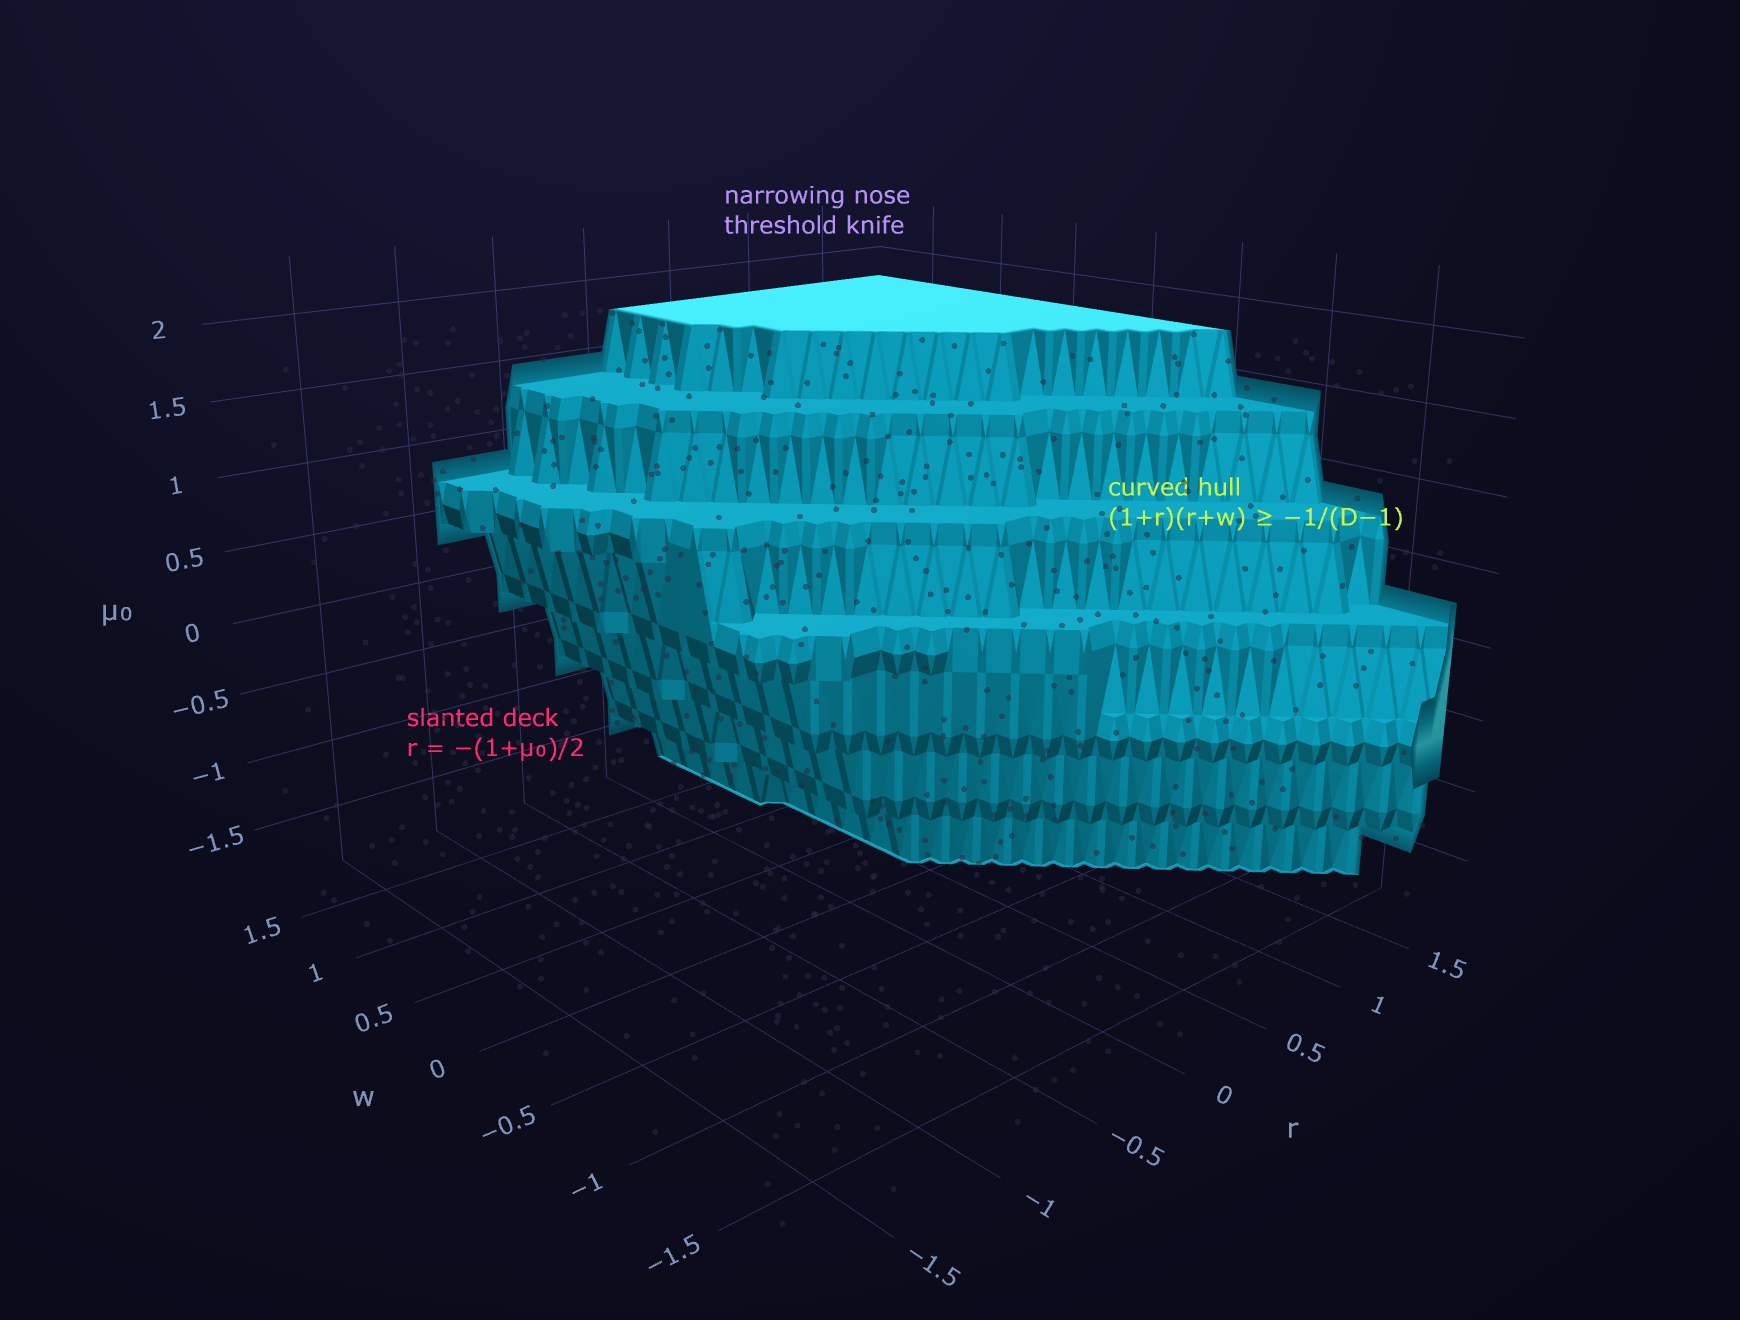
\includegraphics[width=0.9\textwidth]{fig_bow3d.png}
\caption{For fun: the companion \emph{open-string} family \cite{us} drawn in
the same style --- the solid of surviving candidates in $(r,w,\mu_0)$, every
voxel an exact rational verdict. The slanted deck is the edge law, the curved
hull the hyperbola $(1{+}r)(r{+}w)\ge-1/(D{-}1)$, and the narrowing nose the
threshold knife of that paper.}
\label{fig:bow}
\end{figure}

\section*{Reproducibility and AI disclosure}
All claim-bearing computations use exact rational arithmetic; the evaluator,
the falsification suites (the adversarial reviewer's seven-battery script
included), all scan artifacts, and the append-only research log are released
with this paper. This research was conducted by the author working with an AI
research assistant (Claude, Anthropic); every derivation passed an
independent adversarial review, and every number in this paper is
regenerated by a single published battery script. During this work an
implementation bug (a Pochhammer increment step, coinciding with the correct
evaluator only at $\lambda=1$) was found, disclosed and fixed in the public
log; all results affected by it were voided and recomputed, and the
$\lambda=1$ results it could not affect were re-verified independently.

\begin{thebibliography}{9}
\bibitem{CHR2024b} C.~Cheung, A.~Hillman and G.~N.~Remmen,
``Uniqueness Criteria for the Virasoro-Shapiro Amplitude,''
Phys.\ Rev.\ D 111, 086034 (2025), arXiv:2408.03362.
\bibitem{CHR2024} C.~Cheung, A.~Hillman and G.~N.~Remmen,
``Bootstrap Principle for the Spectrum and Scattering of Strings,''
Phys.\ Rev.\ Lett.\ 133, 251601 (2024), arXiv:2406.02665.
\bibitem{us} A.~Pluzhnik, ``The Island Has Edges,'' DOI 10.5281/zenodo.21934462.
\end{thebibliography}
\end{document}
